\section{AD Wandler}\hartl{475}
\subsection{Lernziele}
\begin{itemize}
  \item Parallelverfahren und Kaskaden umsetzer
  \item Wägeverfahren und dessen schaltungstechnische Implementierung
  \item Integrierende und zählende Umsetzer
  \item eigenschaften und Anwendungsgebiete der unterschidlichen Verfahren
\end{itemize}

\subsection{Parallelverfahren und Kaskadenumsetzer}
\begin{longtable}{|l|l|l|}
\hline
\textbf{Parallelumsetzer}\hartl{478}
&
\begin{minipage}{6cm}
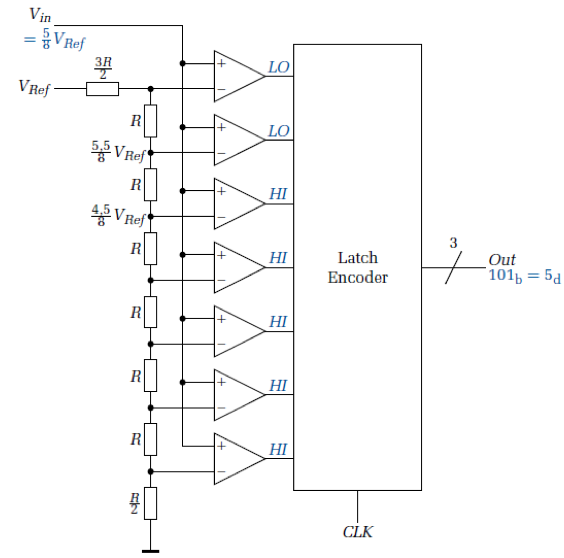
\includegraphics[width=6cm, height = 6cm]{pictures/parallelADC}
\end{minipage}
&
\begin{minipage}{6cm}
\begin{itemize}
  \item sehr schnell
  \item $2^n$ Widerstände
  \item $2^n$ Komparatoren
\end{itemize}
\begin{equation}
Anz_{Vergleiche}=2^N-1
\end{equation}
\end{minipage}\\
\hline

\textbf{Kaskadenumsetzer}\hartl{479}
&
\begin{minipage}{7cm}
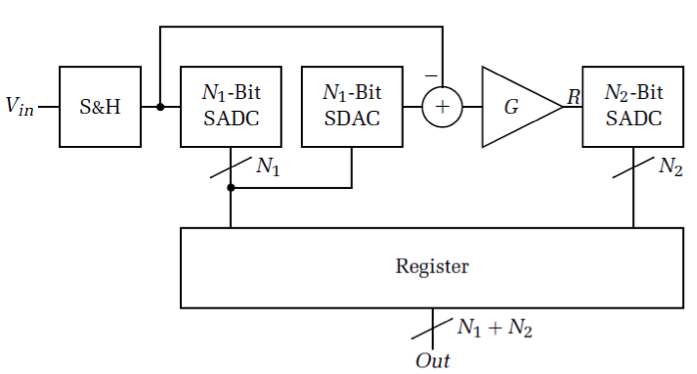
\includegraphics[width=7cm, height = 6cm]{pictures/kaskaden}
\end{minipage}
&
\begin{minipage}{6cm}

Eine 10-bit-Auflösung beim Parallelverfahren würde 1024 Komperatoren
benötigen.$\Rightarrow$Komplexitätsreduktion \\

Mit erstem $N_{1}$-bit ADU wird der Grobbereich festgelegt (höherwertige Bits).
Diese Zahl wird in eine analoge Spannung durch einen $N_{1}$-bit DAU zurück
umgesetzt und diese Spannung von der Eingangsspannung subtrahiert. Diese
Differenz wird von einem weiteren $N_{1}$-bit-ADU umgesetzt, um die
niederwertigen Bits zu ergeben. Skaliert man die Differenzspannung mit dem Faktor 32, hat man
den gleichen Spannungsbereich, kann also zwei identische ADU benutzen.\\
\end{minipage}\\
\hline
\textbf{Pipelined ADC}\hartl{483}
&
\begin{minipage}{7cm}
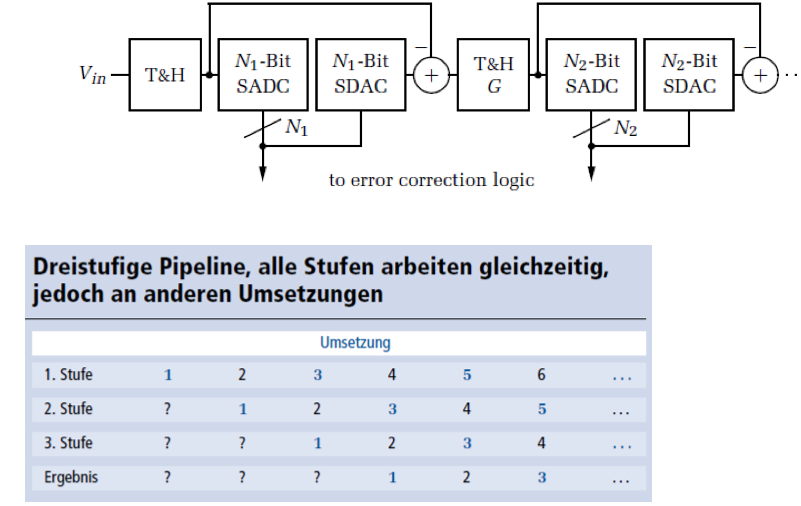
\includegraphics[width=7cm, height = 6cm]{pictures/pipelined}
\end{minipage}
&
\begin{minipage}{6cm}
\begin{itemize}
  \item fast gleiche hohe Umsetzrate wie Parallelumsetzer
  \item gleicher schaltungstechnischer Aufwand wie beim Kaskadennumsetzer
  \item wird heute für schnelle ADC's verwendet
\end{itemize}
\end{minipage}\\
\hline
\end{longtable}


\subsection{Wägeverfahren ( sukzessive Approximation)}\hartl{485}
\begin{itemize}
  \item guter Kompromiss zwischen benötigter Umsetzzeit und erreichbarer
  Auflösung
\end{itemize}

\begin{longtable}{|l|l|l|}
\hline
\begin{minipage}{4cm}
\textbf{Prinzip}\hartl{485}
\end{minipage}
&
\begin{minipage}{6cm}
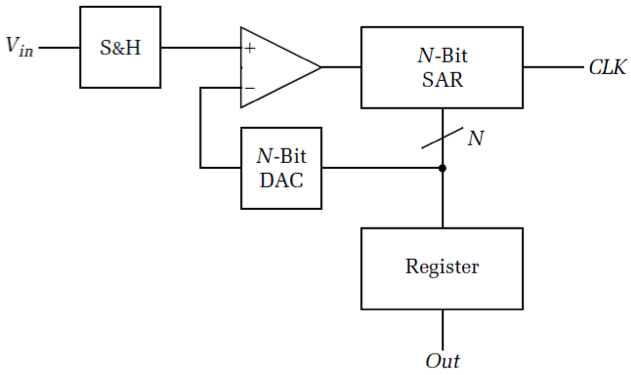
\includegraphics[width=6cm, height = 4cm]{pictures/waegeverfahren}\\
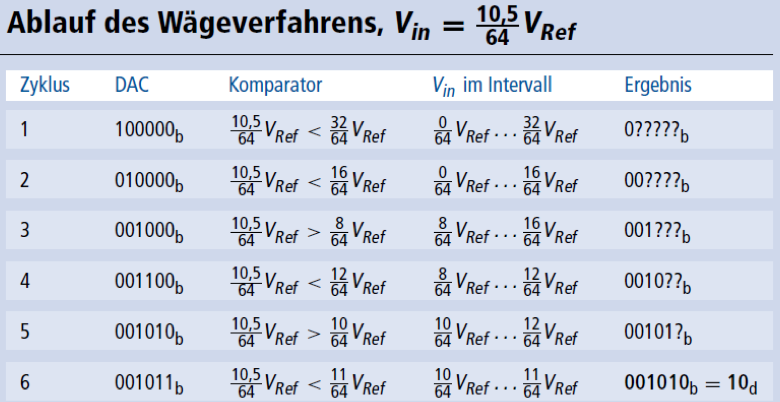
\includegraphics[width=6cm, height = 3cm]{pictures/waegeverfahrentabelle}
\end{minipage}
&
\begin{minipage}{8cm}
\begin{itemize}
  \item Abtastung der Eingangsspannung $V_{in}$mit einer
  S\&H-Schaltung( Vergleichsspannung liegt so während der gesamten Umsetzung an)
  \item Vergleich starte in der Mitte der Eingangsspannung $\frac{V_{Ref}}{2}$
\end{itemize}
\end{minipage}
\\
\hline
\begin{minipage}{4cm}
\textbf{Wägeverfahren mit SC-Prinzip}\hartl{488}
\end{minipage}
&
\begin{minipage}{6cm}
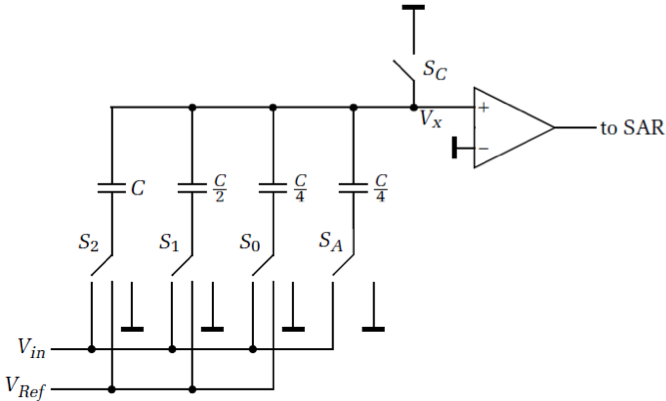
\includegraphics[width=6cm, height = 4cm]{pictures/waegeverfahrenSC}\\
\end{minipage}
&
\begin{minipage}{8cm}
\begin{itemize}
  \item häufig eingesetze Implementierung
  \item mit geschalteten Kapazitäten ist es möglich Halte-Glied und DAc in einer
  Schaltung zu realisieren
\end{itemize}
\begin{enumerate}
  \item Schalter $S_{2},S_{1},S_{0},S_{A}$ verbunden mit $V_{in}$ und $S_{C}$mit
  GND$\to$ alle Kapazitäten werden auf $V_{in}$aufgeladen
  \item öffnen der Schalter $S_{C}und S_{A}$ und bleiben in dieser Stellung
  \item $S_{2}$ auf $V_{Ref}$ und $S_{1},S_{0}$auf GND $\to$
  $V_{x}=-V_{in}+0,5V_{Ref}$
  \item Ergebnis von SAR ausgewertet $\to$ $S_{2}$bleibt oder wechselt auf GND
  \item Fortzetung mit den folgenden Schaltern
\end{enumerate}
\end{minipage}
\\
\hline
\begin{minipage}{4cm}
\textbf{Iterative ADC}
\end{minipage}
&
\begin{minipage}{6cm}
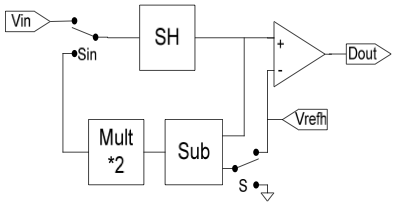
\includegraphics[width=6cm, height = 3cm]{pictures/iterativeADC}
\end{minipage}
&
\begin{minipage}{8cm}
\begin{enumerate}
  \item Im S/H wird die Eingangsspannung geschpeichert (Schalter Sin)
  \item Schalter Sin wird danach auf den Multiplizierer-Ausgang geschaltet
  \item X(Laufvariable) wird auf n-1 gesetzt
  \item Der Jomparator wird ausgewertet\\
  Dout=1: Bx=1, Switch S=1 (d.h. im Subtrahierer wird Vrefh von Vc
  subtrahiert)\\
  Dout=0: Bx=0, Switch S=0 (d.h. im Subtrahierer wird 0 von Vc
  subtrahiert)
  \item Der Subtrahierer generiert sein Ausgangssignal
  \item Der Multiplizierer generiert sein Ausgangssignal
  \item Im S/H wird die Feedback-Spannung gespeichert (Schalter Sin)
  \item X wird um 1 reduziert
  \item Gehe zu Schritt 4, wenn $X\geq0$
\end{enumerate}
\end{minipage}
\\
\hline
\end{longtable}



\subsection{Zählverfahren}\hartl{490}
Ist für kontinuierliche Auswertungen des Eingangssignal
\begin{longtable}{|l|l|l|}
\hline
\begin{minipage}{4cm}
\textbf{Single Slope}
\end{minipage}
&
\begin{minipage}{6cm}
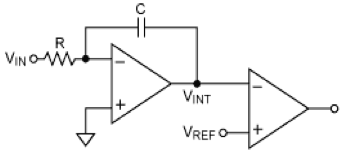
\includegraphics[width=6cm, height = 4cm]{pictures/singleSlope1}\\
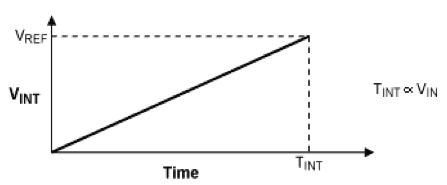
\includegraphics[width=6cm, height = 3cm]{pictures/singleSlope2}
\end{minipage}
&
\begin{minipage}{8cm}
\begin{equation}
T_{int}=\frac{V_{Ref}*R*C}{V_{in}}
\end{equation}
\end{minipage}
\\
\hline
\begin{minipage}{4cm}
\textbf{Dual Slope}\hartl{492}
\end{minipage}
&
\begin{minipage}{6cm}
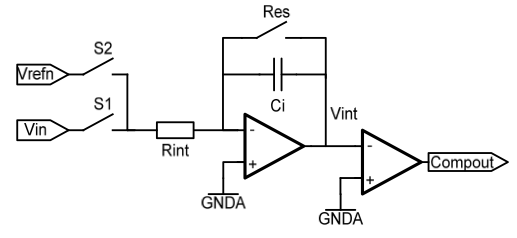
\includegraphics[width=6cm, height = 4cm]{pictures/dualSlope11}\\
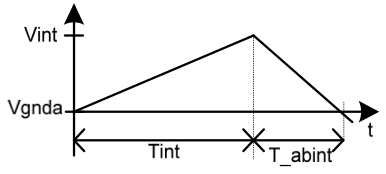
\includegraphics[width=6cm, height = 3cm]{pictures/dualSlope12}\\
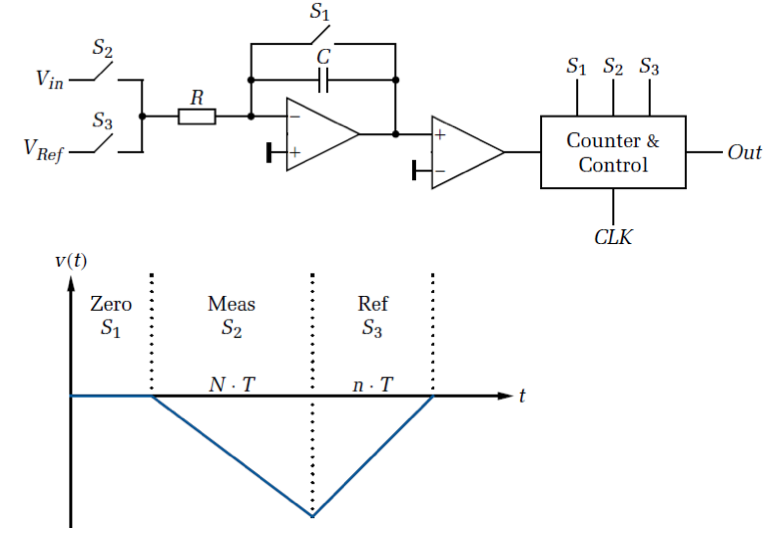
\includegraphics[width=6cm, height = 5cm]{pictures/dualSlope2}
\end{minipage}
&
\begin{minipage}{8cm}
\begin{gather}
V_{int}=
\int^{V_{int}}_{0}\frac{-1}{R_{int}*C_{i}}*(V_{in}-V_{GNDA})dt+V_{GNDA}\\
V_{intmax}=\frac{-1}{R_{int}*C_{i}}(V_{in}-V_{GNDA})*T_{int}+V_{GNDA}\\
V_{int}(t)=V_{intmax}-\frac{-1}{R_{int}*C_{i}}(V_{in}-V_{GNDA})*t\\
t_{abint}=\frac{-(V_{in}-V_{GNDA})*T_{int}}{V_{refn}-V_{GNDA}}\\
\int^{NT}_{0}V_{in}dt=NTV_{in}\\
NTV_{in}-\int^{nT}_{0}V_{Ref}dt=NTV_{in}-nTV_{Ref}=0\\
n=\frac{V_{in}}{V_{Ref}}N\\
n=\frac{RCV_{off,C}-TV_{off,OP}}{T(V_{Ref}+V_{off,OP})}+N\frac{V_{in}}{V_{Ref}+V_{off,OP}}
\end{gather}
\begin{tabular}{ll}\\
N:&Taktzyklen\\
T:&Periodendauer\\
n:&Zählerstand\\
$V_{off}$:&Offsetspannung\\
\end{tabular}
\end{minipage}
\\
\hline
\begin{minipage}{4cm}
\textbf{Spannungs- Frequenz- Umsetzer}\hartl{495}
\end{minipage}
&
\begin{minipage}{6cm}
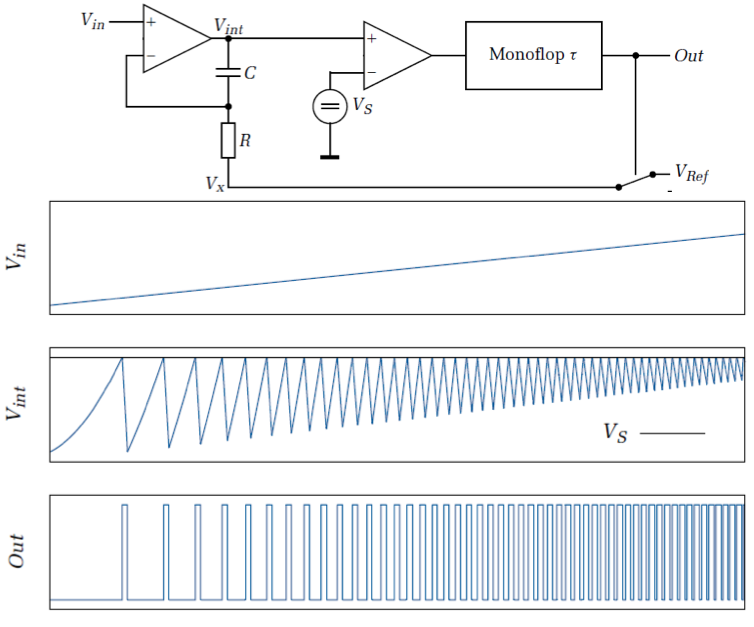
\includegraphics[width=6cm, height = 4cm]{pictures/sfu}
\end{minipage}
&
\begin{minipage}{8cm}
\begin{equation}
V_{int}(t)=V_{in}+\frac{1}{RC}\int(V_{in}-V_{x})dt
\end{equation}
Vorteil: Immer am Eingangssignal\\
Nachteil: Kein echter ADC\\
\end{minipage}
\\
\hline
\begin{minipage}{4cm}
\textbf{Ladungs-Ausgleichs-Integrator}\hartl{497}
\end{minipage}
&
\begin{minipage}{6cm}
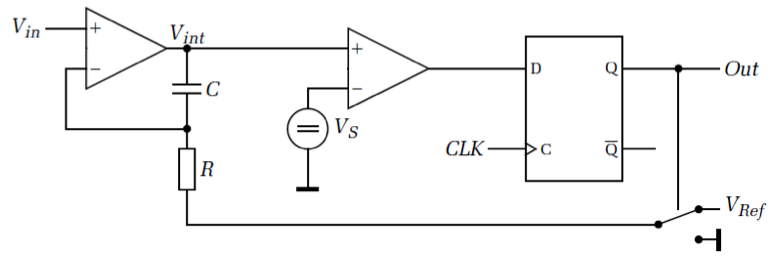
\includegraphics[width=6cm, height = 4cm]{pictures/lsg1}\\
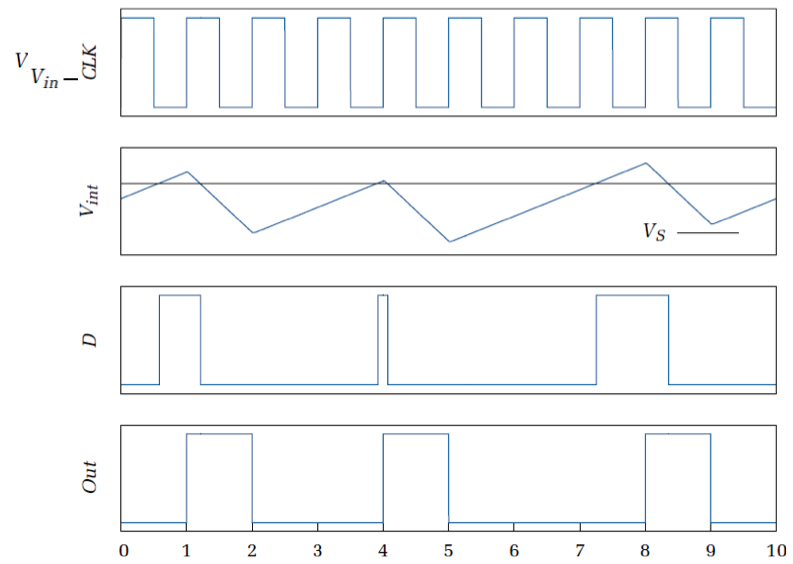
\includegraphics[width=6cm, height = 3cm]{pictures/lsg2}
\end{minipage}
&
\begin{minipage}{8cm}
\begin{itemize}
  \item Gleichgewichtsbedingung\\
  \begin{equation}
  V_{in}-\frac{n}{N}V_{Ref}=0\Rightarrow n=\frac{V_{in}}{V_{Ref}}N
  \end{equation}
\item Flipflop statt Monoflop
\end{itemize}
\end{minipage}
\\
\hline
\begin{minipage}{4cm}
\textbf{Sigma-Delta Wandler}\hartl{500}
\end{minipage}
&
\begin{minipage}{6cm}
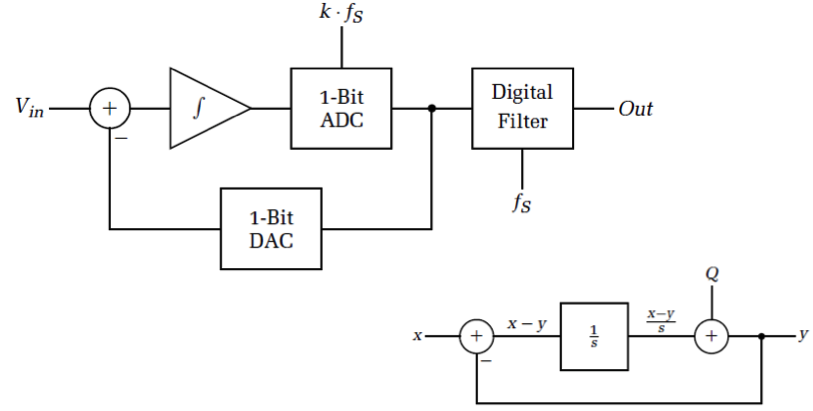
\includegraphics[width=6cm, height = 4cm]{pictures/deltaSigma1}
\end{minipage}
&
\begin{minipage}{8cm}
\begin{itemize}
  \item Ersatzschaltung für Frequenzbereich
  \item Tiefpass für Signal
  \item Hochpass für Q
\end{itemize}
\begin{equation}
y=\frac{x-y}{s}+Q\Rightarrow y=x\frac{1}{1+s}+Q\frac{s}{1+s}
\end{equation}
\end{minipage}
\\
\hline
\begin{minipage}{4cm}
\textbf{Sigma-Delta Wandler 2. Ordnung}\hartl{502}
\end{minipage}
&
\begin{minipage}{6cm}
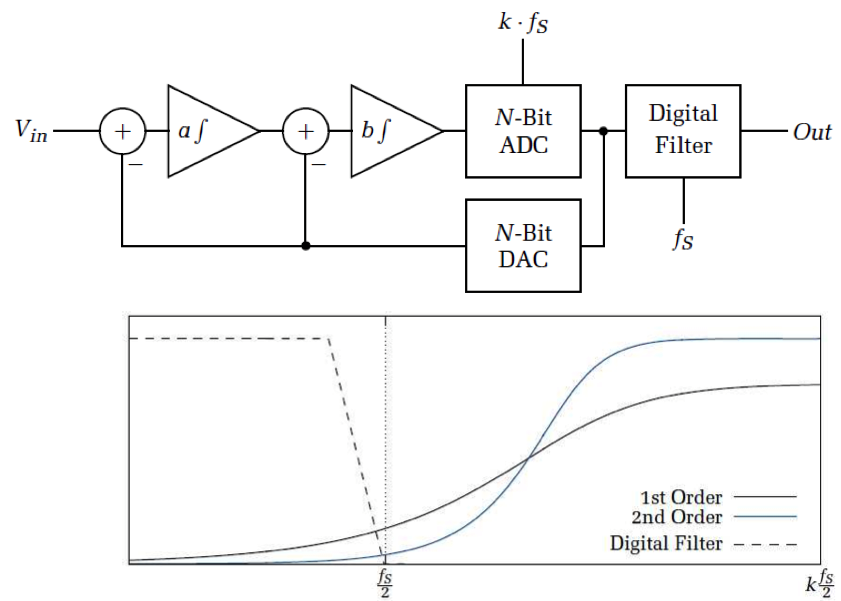
\includegraphics[width=6cm, height = 4cm]{pictures/deltaSigma2}
\end{minipage}
&
\begin{minipage}{8cm}

\end{minipage}
\\
\hline
\end{longtable}




\subsection{Kennwerte von ADC's}
\begin{figure}[!htbp]
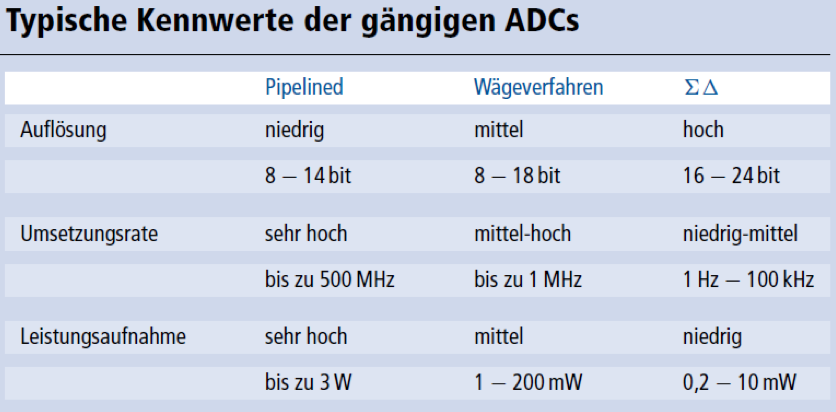
\includegraphics[scale=0.4]{pictures/kennwerteADC}
\end{figure}

\subsubsection{Aufwand Wandlertypen}
\begin{figure}[!htbp]
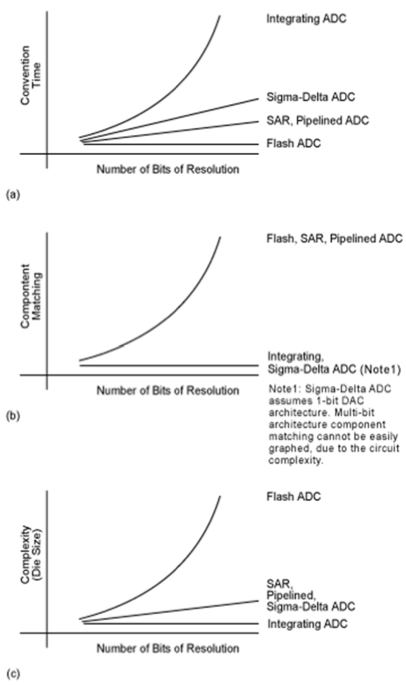
\includegraphics[scale=0.5]{pictures/aufwandWandler}
\end{figure}
